\documentclass{svproc}
\usepackage[T1]{fontenc}
\usepackage[utf8]{inputenc}
\usepackage{newtxtext,newtxmath}
\usepackage{graphicx,amsmath,booktabs,array,url,flafter}
\usepackage[hidelinks]{hyperref}
\hypersetup{pdftitle={Explaining Narrative Events with Generative AI and Structural Causal Models},pdfauthor={},pdfsubject={},pdfkeywords={},pdfcreator={},pdfproducer={}}
\pdfinfoomitdate=1
\pdftrailerid{}
\graphicspath{{../../figures/publication/}}
% Reusable short captions. Provenance and qualifications belong in the text.
\newcommand{\CrowCaption}{Causal map of the Crow and the Pitcher, showing alternative routes to water reachability in the controlled story.}
\newcommand{\BlackwaterCaption}{Fuel deployment, ignition and fleet exposure combine in the Blackwater wildfire mechanism, separating preparation from implementation and immediate damage.}
\newcommand{\RedWeddingCaption}{Prepared attackers and guest attendance converge on the Red Wedding ambush; grievance and perceived protection have distinct roles.}
\newcommand{\BoltonCaption}{Encirclement and relief at Winterfell: (a) the local mechanism; (b) intervention outcomes under two assumptions about the subsequent advance.}
\newcommand{\AstaporCaption}{The Astapor sequence connects (a) purchase and command transfer with (b) armed action, emancipation and departure with freed troops.}
\newcommand{\HumptyCaption}{Damage, attempted repair and effective repair remain distinct in the controlled Humpty Dumpty story; successful repair removes remaining damage.}
\newcommand{\WolfCaption}{Credibility and a new warning jointly determine timely response in the controlled Wolf story; timely response prevents flock harm.}

% Generated by scripts/build_narrative_paper.py from results/v2/test_summary.json.
% Archive SHA256: 03036b8f44c63d0d6c86ce208b4e0b2001079ffa5f8aacbd024005f521ad7a9e
\newcommand{\ExecutionGain}{21.0}
\newcommand{\ExecutionLower}{9.6}
\newcommand{\ExecutionUpper}{32.8}
\newcommand{\BenchmarkTable}{%
\begin{tabular}{@{}lrr@{}}
\toprule
Method & Identified (\%) & Changing (\%) \\
 & 72 SCMs & 40 SCMs \\
\midrule
Direct answers & 56.7 & 54.6 \\
Synthesis and execution & 77.8 & 80.0 \\
Factual carry-forward & 86.2 & 0.0 \\
\bottomrule
\end{tabular}
}

\newcommand{\doop}{\operatorname{do}}
\newcommand{\Pa}{\operatorname{Pa}}
\newcommand{\ep}[1]{\textup{#1}}
\typeout{PAPER-TEXTWIDTH: \the\textwidth}
\typeout{PAPER-TEXTHEIGHT: \the\textheight}
\begin{document}
\mainmatter
\raggedbottom
\title{Explaining Narrative Events with Generative AI and Structural Causal Models}
\titlerunning{Explaining Narrative Events}
\author{}
\authorrunning{}
\institute{}
\maketitle

\begin{abstract}
Interconnected narratives distribute explanations across actions, beliefs, resources and earlier decisions. A chronological summary can recover what happened while leaving unclear how these elements worked together. We present a method that combines generative AI interpretation with structural causal models to construct readable, inspectable causal maps. Generative models propose meaningful events, intermediate steps and passage-linked explanations. Structural equations specify how conditions combine, and partial functions preserve behavior left unspecified. Interventions change selected events and propagate their consequences through fixed mechanisms. A worked Crow and the Pitcher example shows why adding stones matters with initially low water but becomes unnecessary when water is already reachable. The principal application comprises six Game of Thrones television cases. Their maps distinguish resources from coordinated action at Blackwater, motivation from opportunity at the Red Wedding, relief from removal of an obstruction at Winterfell, and command from voluntary service at Astapor. Six of 18 application questions distinguish the two scenario models considered in each case. A separate controlled-text benchmark supports synthesis followed by execution over direct answering, particularly on outcome-changing questions. The contribution connects source passages, readable relationship descriptions and executable joint mechanisms. Readers can trace an explanation, inspect how influences converge and locate the assumptions responsible for different hypothetical outcomes.
\keywords{narrative explanation, generative AI, structural causal models, causal maps, counterfactual reasoning}
\end{abstract}

\section{Introduction}
An explanation of a narrative event often depends on more than its immediate predecessor. A battle can turn on an available resource, the decision to deploy it, a signal, an effective action and the opponent's exposure. A betrayal can depend on grievance, protection from retaliation and the victims' presence. These elements may appear in different scenes and involve different characters. Bringing them together requires interpretation; specifying how they work together requires a representation of their joint mechanism.

Generative AI offers a way to organize this material. It can identify event meanings, connect references across passages, propose intermediate steps and describe how one event creates an opportunity for another. A readable causal map preserves these proposals as inspectable relationships. Structural causal models (SCMs) add a complementary capability: they state how an event depends on its parents and on contextual conditions, so that a hypothetical change has a defined consequence \cite{pearl2009}. An arrow then carries both a narrative explanation and a role in a local mechanism.

The contribution is a causal map in which each relationship connects a passage-based interpretation to an executable mechanism. A reader can follow why an event matters, inspect how it combines with other conditions, and change one condition to see what follows. Informative edge descriptions explain the process; joint equations distinguish requirements from alternative routes; interventions reveal which conclusions depend on additional assumptions. This combination goes beyond listing events or drawing causal arrows. It also keeps evidence that an event occurred separate from evidence for an influence and from assumptions about its exact function.

The television narrative of \emph{Game of Thrones} makes these questions concrete. Character and faction stories intersect across episodes: acquiring a resource creates a later military opportunity, a broken alliance changes the risks of betrayal, and a request for assistance shapes a subsequent battle. Beliefs, grievances, resources and timing work together rather than in isolation. Six local case studies examine particular outcomes within this larger narrative. Blackwater connects an earlier acquisition to a coordinated trap; the Red Wedding connects motivation and protection to access to the victims; Winterfell separates an obstruction from its removal; and Astapor follows command into armed action and voluntary service. These cases offer several complementary explanations, rather than a series-wide causal graph.

A worked example introduces the equations before the television application. A separate controlled benchmark tests execution on explicit rules.

\section{Motivating Example: The Crow and the Pitcher}\label{sec:crow}
A thirsty crow finds water below its reach, adds stones, raises the water and drinks. For a controlled reference example, an original retelling adds explicit rules about stone availability, an intact pitcher and initial reachability. These rules specify a small mechanism rather than relying on every reader to supply the same unstated physical assumptions.

Let $S$ mean that enough stones are available, $I$ that the pitcher is intact, and $B$ that the water is initially reachable. Let $A$ denote adding enough stones, $R$ raising the water, $T$ water being reachable after the action, and $D$ drinking. Each variable is Boolean: one means that the defined event occurs or condition holds. Sufficient water and the crow's readiness to act and drink are held fixed. The specified rules are
\begin{equation}\label{eq:crow}
 A=S,\qquad R=I\land A,\qquad
 T=I\land(B\lor R),\qquad D=T.
\end{equation}
Here $\land$, $\lor$ and $\neg$ mean conjunction, disjunction and negation. Thus adding stones raises the water in the intact pitcher. Water is reachable either because it was reachable initially or because it has been raised, provided the pitcher retains access. Drinking follows reachability within the stated context. Figure \ref{fig:crow} gives these rules readable event and relationship labels.



\begin{samepage}
The factual inputs are $S=I=1$ and $B=0$. Executing the equations gives $A=R=T=D=1$. Now prevent stone addition, keeping the water initially low. Replacing the first equation by $A=0$ gives $R=T=D=0$: the crow cannot drink through the represented route. In a contrasting intervention, prevent addition and make the water initially reachable, setting $A=0$ and $B=1$. Then $R=0$ but $T=D=1$. The same prevented action has different consequences because the second route to reachability remains available.
\par
\end{samepage}

\begin{figure}[htb]
\centering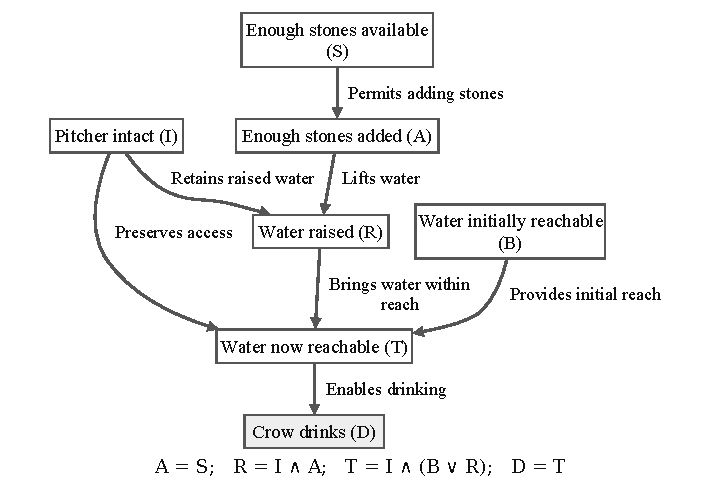
\includegraphics[width=\linewidth]{simple_stories/crow.pdf}
\caption{\CrowCaption}\label{fig:crow}
\end{figure}

The map therefore explains more than the sequence ``stones, rising water, drinking.'' It distinguishes an action from its intermediate physical effect and separates that effect from an already-satisfied condition. Stones are required for drinking in the first context, but not in every context admitted by the model. The joint reachability equation makes this distinction precise. Additional controlled reference examples in Appendices \ref{app:humpty} and \ref{app:wolf} illustrate repair and credibility mechanisms.

\section{Related Work}
Narrative representations have long organized events around participants and time. Chambers and Jurafsky's narrative event chains connect events sharing a protagonist and learn partial temporal order \cite{chambers2008}. Elson et al. extract literary social networks from dialogue interactions \cite{elson2010}. These reveal event regularities and character relationships. An intervention requires an additional commitment: specifying how the consequence changes when an input is altered. Our maps attach that joint mechanism to meaningful events, decisions, beliefs and resources.

Recent work directly constructs causal graphs from narratives. Li et al. extract agent-centered events, use linguistic features to classify narrative roles, and iteratively refine a connected graph \cite{li2025}. Koupaee et al. combine language-model experts for different semantic relations and use the resulting graphs for event forecasting and reasoning \cite{koupaee2025}. Our contribution addresses a further representational question: what joint rule makes the incoming relationships produce their child event? Two arrows can support either complementary requirements or substitute routes, with different intervention answers. We connect their natural-language explanations to finite functions, preserve unspecified behavior, and execute changes while holding the other mechanisms fixed. This supplies an inspectable account of the assumptions behind an answer, alongside the causal connections emphasized in those studies.

Generative knowledge construction also motivates the division of labor. COMET generates commonsense descriptions \cite{bosselut2019}. Such knowledge can suggest a question or missing step, but a narrative interpretation must be checked against its source. Program-aided language models delegate calculation to an interpreter after generating a program \cite{gao2023}. We similarly separate interpretation from execution, while preserving the program as a passage-linked mechanism that readers can inspect.

SCMs supply intervention semantics \cite{pearl2009}. Bynum and Cho's sequence-driven SCMs combine user-defined structure with language-model-defined mechanisms to generate observational, interventional and counterfactual data \cite{bynum2025}. Here generative interpretation also proposes event meanings and dependencies; the resulting finite functions are checked against their descriptions and sources. Neither causal graph generation nor structural modeling is new. Our contribution connects a passage-based interpretation to the joint rule responsible for a computed consequence, with visible alternatives where the encoding is incomplete.

\section{Methodology}\label{sec:method}
\subsection{From passages to mechanism records}
Construction begins by specifying an outcome, time interval and explanatory boundary. ``The assault is repelled by the end of the battle'' differs from ``the enemy fleet suffers severe losses.'' A useful variable states which event occurs, for whom, and by when. Its record includes an operational definition, domain, actor, event time, factual state and passage references. Reports and beliefs are distinguished from the external events they concern; the episode containing a retrospective report need not be the time of the reported event.

The source collection is broader than the initial model context. Episodes are organized into locatable passage containers. Retrieval first covers relevant actors, events and decisions; generation then proposes questions about missing connections. These questions search the broader case corpus, and surrounding passages are read before accepting a relationship. A proposed mechanism can therefore trigger further retrieval, splitting of a conflated variable, insertion of a supported mediator, correction of temporal scope or retraction of an unsupported connection. Chronological succession alone does not establish a causal edge.

Each proposed edge retains a short graphical phrase and a fuller process description. The record identifies conditions, qualifications, supporting passages, what each passage supports, contradictory material and unresolved gaps. A relationship may be explicitly stated, contextually inferred, hypothetical, contradicted or unresolved. This description governs construction: a distinction between permission and action, for example, can require two variables before an equation is chosen. Children with several parents also receive a joint description of how those influences combine.

Three judgments remain separate. A passage can establish that an event occurred; it can support a directional influence; and it can constrain a particular functional form. Evidence for the first two does not automatically establish the third. ``Helps'' and ``enables'' need contextual interpretation, whereas ``is necessary'' or ``exactly when'' makes a stronger, testable commitment. Short labels communicate the process; the accompanying record carries its qualifications.

\subsection{Explicit mechanisms and interventions}
For each endogenous event or state $X_i$, the structural specification is
\begin{equation}\label{eq:scm}
 X_i=f_i(\Pa_i,U_i).
\end{equation}
Here $\Pa_i$ is the collection of parent events represented in the graph, $U_i$ contains contextual inputs, and $f_i$ is the local mechanism. The present models use finite, principally Boolean domains and an acyclic dependency graph. The equations express whether a defined event occurs or condition holds. They are constructed rules, not statistical regression equations fitted to repeated observations.

An intervention $\doop(X_k=x)$ replaces the equation or input assignment for $X_k$ by the constant $x$. Other functions and the factual background remain fixed. For example, $\doop(A=0)$ in the Crow model replaces $A=S$ while retaining the rise, reachability and drinking rules. With $I=1$ and $B=0$, the change propagates through $R$ and $T$ to $D=0$. A joint intervention replaces more than one assignment at once, as in $\doop(A=0,B=1)$.

Several incoming arrows require a joint rule. In Eq. \ref{eq:crow}, the intact pitcher and stone addition are jointly required for the represented rise, whereas initial reachability and raised water provide alternative routes to reachability. Inhibition is represented by a negated condition, as when timely relief prevents an encirclement from persisting. An event can therefore contribute by supplying an input, completing a conjunction, providing a substitute route or removing an obstruction. Execution follows these mechanisms through intermediate events and convergence points. It evaluates a shared event once, even when several explanatory paths pass through it; the present application attaches neither probabilities nor additive responsibility weights to those paths.

\subsection{Preserving incomplete mechanisms}
A narrative often depicts only one combination of inputs, whereas an executable function covers other combinations too. The representation can leave these unencoded configurations unspecified. It then represents a family of functions satisfying the encoded evidence constraints and additional assumptions, rather than inventing a complete rule. Execution can evaluate one explicit scenario, enumerate a small family, or search a larger family with stated coverage. Appendix \ref{app:uncertainty} defines the outcome sets and distinguishes complete results from sampled possibilities.

The broad application families deliberately fix factual input-output rows while leaving many unobserved rows free. They are conservative sets of possible mechanisms under that encoding, not complete formalizations of everything a passage might imply. An unresolved answer therefore describes the encoded constraints. It can reflect missing formalization as well as uncertainty in the narrative; these are different diagnoses. Complete scenarios add explicit assumptions so that readers can explore their consequences. Two scenarios may reproduce the same battle while giving reinforcements different counterfactual roles. Their generation frequencies are not probabilities, and agreement among sampled candidates alone does not establish that every compatible function gives the same answer.

\subsection{Consistency, refinement and presentation}
The workflow checks three links: source to description, description to function, and function to reported result. Source checking combines passage-location verification with contextual semantic review. For small finite mechanisms, formal claims can be checked over all input configurations. If a parent is asserted to be necessary, every configuration in which that parent is absent must make the child absent. Examining only the all-zero row is insufficient. A violated proposition yields a concrete counterexample. An unspecified row compatible with both outcomes instead identifies an encoding gap, unless the retained constraints exclude the prose claim altogether.

Discrepancies lead to a limited revision, rejection or an unresolved status, with original proposals preserved. Established facts cannot be relaxed to obtain an executable model. Prose explanations receive computed states and outcomes. Mechanical checks verify those values; semantic review considers interpretation and source support.

The application used Qwen3-14B-AWQ for source-grounded proposals and retrieval questions. A Codex assistant subsequently read source packets and adjacent context, constructed the final mechanisms and scenario equations, and recorded revisions. The final application models are assistant-refined syntheses, distinct from the initial generator outputs. Both stages used general modeling instructions, without a researcher-supplied Game of Thrones graph or fixed story equations.

Figures render accepted mechanism records. Solid edges denote explicitly supported directional relationships; dashed edges denote contextual interpretations. Neither style certifies an exact Boolean function. Compact equations state the scenario being examined, and fuller conditions and references appear in the mechanism catalogue. Detail views show a local mechanism; conclusions about a later outcome use the complete model, whose additional mechanisms are described where needed. Mathematical symbols are local to each case.

\subsection{A construction trace: the Blackwater trap}\label{sec:construction}
The wildfire sequence illustrates the full process. In the source collection \cite{screenscripts}, \ep{S02E05}, passage S15, establishes Tyrion's control of the supply. In \ep{S02E09}, S14 describes its release from a ship; S15 describes Tyrion's torch signal and Bronn's flaming arrow; S16 and S19 describe ignition and fleet losses. These passage identifiers are the transcript's scene and line locators, including S15L1 for the signal-and-arrow sequence. They make each part of the proposed mechanism recoverable from a small passage set.

The initial Qwen proposal identified Tyrion's decision to control wildfire and its defensive use, but a subsequent source pass incorrectly assigned the arrow to Tyrion. The recorded refinement checked S15 against the adjacent action. It separated signal giver from archer, inserted deployment between supply and damage, and limited the damage claim because S21 shows Stannis surviving and ordering a landing. The resulting variables preserve these distinctions throughout the explanation and calculation.

The final mechanism description states that released wildfire carries ignition through the trap area and burns exposed vessels. Let $W$ denote supply under Tyrion's control, $T$ deployed fuel, $S$ his signal, $I$ Bronn's ignition, $B$ fleet exposure and $D$ severe fire losses. The complete scenario specifies
\begin{equation}\label{eq:blackwater}
 T=W,\qquad I=S,\qquad D=T\land I\land B.
\end{equation}
The deployment decision, a prepared archer and absence of substitute ignition are fixed background assumptions. The passages establish the depicted actions; the scenario supplies the stronger joint rule needed to test their absence. Under $\doop(I=0)$, fuel and exposure stay in place but $D=0$. Both complete battle scenarios still repel the assault through other modeled actions (Section \ref{sec:blackwater}). Generative interpretation supplies event distinctions and explanations; refinement checks their actors and scope; deterministic execution computes consequences with the mechanisms fixed.

\section{Study Design and Narrative Material}\label{sec:design}
\subsection{Television case studies}
The application corpus comprises 41 episode pages and 924 scene containers from a single accessible, unofficial transcription collection \cite{screenscripts}. Containers can cover several locations and serve as retrieval units, rather than necessarily coherent causal episodes. Records preserve episode identifiers, passage boundaries, source URLs and content hashes. Dialogue and stage descriptions are interpreted in their surrounding context. This study uses television continuity throughout; a later report can support an earlier event without becoming its cause.

Table \ref{tab:cases} defines the six endpoints. They span mobilization, betrayal, battle outcomes and a military departure. Their 69 variable records and 71 relationships include related events across cases; the six interpretive case studies are not independent statistical samples. Each case has a partial mechanism graph, two functionally distinct complete scenarios and three questions selected before computing their answers. The four main application figures offer complementary explanatory content, while the full portfolio covers every attempted case.

\begin{table}[htbp]
\caption{Six television case studies and their principal explanatory mechanisms.}\label{tab:cases}
\centering\small
\begin{tabular}{@{}>{\raggedright\arraybackslash}p{.19\linewidth}>{\raggedright\arraybackslash}p{.37\linewidth}>{\raggedright\arraybackslash}p{.38\linewidth}@{}}
\toprule
Case / endpoint & Outcome & Principal mechanism \\
\midrule
Stark-Lannister \newline \ep{S01E07} & Tywin orders Jaime's field deployment against the Riverlands & Allegation and detention connect to a dynastic response; a royal challenge is an alternative influence. \\
Northern coalition \newline \ep{S01E09} & Robb's host crosses the Twins with Frey support & Mobilization supplies a host; negotiated commitments secure permission and assistance. \\
Blackwater \newline \ep{S02E09} & Stannis's assault on King's Landing is repelled & A fire trap, a rear sortie and arriving relief provide interacting military routes. \\
Red Wedding \newline \ep{S03E09} & Robb's leadership and accompanying host are destroyed at the Twins & Concealed preparation and guest presence converge in attacks on the hall and camp. \\
Bolton campaign \newline \ep{S06E09} & The Stark coalition takes Winterfell from Ramsay & Encirclement, timely relief, pursuit and a gate breach connect the field battle to capture. \\
Astapor \newline \ep{S03E04} & Daenerys departs with freed Unsullied after breaking the masters' immediate armed control & Command transfer enables military action; freedom and the decision to remain define the departing force. \\
\bottomrule
\end{tabular}
\end{table}

\subsection{Controlled material and experimental resources}
The short-story checks use frozen retellings and controlled adaptations. Reference equations and four intervention answers per controlled story were specified before generation and withheld from it. Appendix \ref{app:assessment} distinguishes generated outputs from the reference illustrations.

An earlier controlled benchmark supplies a reference for intervention correctness. Its texts are generated from 120 independently constructed SCMs by expressing their rules in explicit language. The split contains 24 development, 24 calibration and 72 held-out models. Four conditions supply complete mechanisms or omit intermediate, outcome or multiple rules. Queries test both determined and underdetermined outcomes under the stated compatible mechanism family. The generating equations and reference answers are withheld from generation and repair feedback. The held-out set contains 1,080 questions, grouped by generating SCM throughout evaluation.

Qwen3-14B-AWQ ran on an NVIDIA RTX 4090 with 24 GB VRAM. The application source passes used 17 requests and 36,659 generated tokens: summed request time was 7.9 minutes, within 31.5 minutes with the inference service running. The simple-story run used 18,814 generated tokens and 6.26 minutes of service time. These are inference timings, excluding subsequent model refinement and analysis. The application assistant's exact served build and token usage were unavailable; its generation route is recorded separately.

\subsection{Controlled execution results}\label{sec:benchmark}
Table \ref{tab:benchmark} compares direct answers with synthesis followed by execution on the same explicit-rule texts. An \emph{identified} question has a single answer across the reference-compatible functions. Accuracy is first calculated over eligible questions within each SCM and then averaged across SCMs. Thus the evaluation unit is the generating model, not an individual question. All 72 test SCMs contribute identified questions; 40 contribute identified questions that change the factual outcome. The 16 syntheses still unsuccessful after repair count as incorrect in the primary execution results.

\begin{table}[htb]
\caption{Model-level intervention accuracy on explicit-rule texts; changing questions require departing from the factual outcome.}\label{tab:benchmark}
\centering\small
\setlength{\tabcolsep}{6pt}
\BenchmarkTable
\end{table}

The paired execution-minus-direct gain is \ExecutionGain{} percentage points, with a 95\% model-level bootstrap interval of \ExecutionLower{} to \ExecutionUpper{} (5,000 paired resamples). The calculation uses unrounded model scores. Outcome-changing questions are especially informative: repeating the factual answer cannot solve a hypothetical change that alters the result. Factual carry-forward performs well overall because outcome preservation is common, yet fails on every changing question. Synthesis followed by execution reaches 80.0\% on that stratum, compared with 54.6\% for direct answers.

This comparison supports the use of synthesized executable rules for controlled text reasoning. Single-model execution, alternative-model execution and the full explanation pipeline have identical identified-answer accuracy, so the gain cannot be assigned to source weighting, rich descriptions or presentation. The benchmark is separate from the television interpretations and short-story checks; it evaluates neither the accuracy of the Game of Thrones mechanisms nor their effect on readers.

\section{Game of Thrones: Results and Interpretation}\label{sec:results}
\subsection{Blackwater: a resource becomes an implemented trap}\label{sec:blackwater}
Possessing wildfire and implementing a coordinated trap make different contributions to the battle. Figure \ref{fig:blackwater} connects Tyrion's acquisition in \ep{S02E05} to deployment and ignition in \ep{S02E09}. The construction trace in Section \ref{sec:construction} explains how those distinctions emerged. Here the phrases ``Supplies fire trap,'' ``Signals the shot'' and ``Ignites the trap'' show why control of a resource, coordination and physical action belong at different points in the explanation.

\begin{figure}[htb]
\centering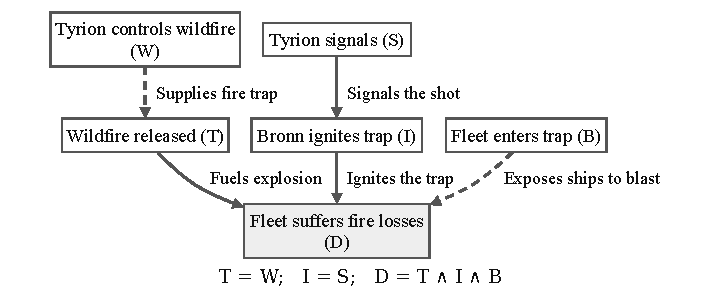
\includegraphics[width=\linewidth]{got/blackwater_mechanism.pdf}
\caption{\BlackwaterCaption}\label{fig:blackwater}
\end{figure}

Equation \ref{eq:blackwater} gives the joint mechanism behind the three incoming arrows to fleet damage. Fuel supplies combustible material, ignition activates it, and exposed ships are the objects damaged. With deployment and archer readiness fixed, supply and signal propagate through distinct implementation steps. Neither a signal without fuel nor fuel without ignition produces the represented damage. The equation makes those complementary roles explicit without collapsing the two actors into a single action.

\begin{samepage}
Fleet damage is distinct from repelling the assault: Stannis survives and continues the attack. The full map therefore includes Tyrion's rear sortie and the later relief force. Preventing Bronn's ignition removes the depicted fire losses but leaves the final assault repelled in both scenarios when the other represented actions occur. Removing relief separates them. One requires relief together with a holding action; the other permits naval attrition and the sortie jointly to substitute. These explicit alternatives locate the assumption behind the final battle answer. The map traces a local tactical contribution without equating it with the whole victory.
\par
\end{samepage}

\subsection{The Red Wedding: preparation meets attendance}
The Red Wedding map separates the motivation to betray from protection for the betrayer, the presence of the victims and preparation to attack them. The material connects the replacement-marriage arrangement in \ep{S03E06}, the wedding in \ep{S03E09}, and the retrospective discussion of protection in \ep{S03E10}. In Fig. \ref{fig:red}, that later report supports an interpretation of earlier assurances; the model places the assurances before the attack.

Let $G$ be Walder Frey's grievance, $A$ Tywin's assurances, $T$ prepared attackers, $N$ acceptance of the replacement marriage, $H$ the promise of guest safety, $P$ the coalition's presence at the wedding, and $X$ the hall ambush. One scenario specifies $T=G\land A$, $P=N\land H$ and $X=T\land P$. A second replaces the preparation rule by $T=A$. The first interpretation makes grievance and protection complementary; the second allows strategic protection to sustain preparation without the represented grievance.

\begin{figure}[htb]
\centering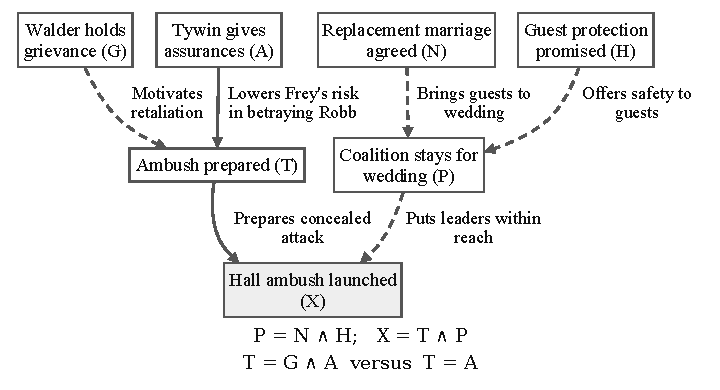
\includegraphics[width=\linewidth]{got/red_wedding_mechanism.pdf}
\caption{\RedWeddingCaption}\label{fig:red}
\end{figure}

The edge about risk concerns \emph{Frey's perceived risk when betraying Robb}. Assurances can reduce anticipated retaliation and thereby support preparation. They are distinct from the guest-safety promise that encourages the intended victims to remain. Likewise, a grievance can motivate retaliation without itself placing the victims within reach. ``Prepares concealed attack'' and ``Puts leaders within reach'' converge on the ambush, exposing the interaction between capability and opportunity.

\begin{samepage}
Removing grievance prevents the final modeled destruction in the first scenario but not the second. Removing assurances prevents it in both. These answers follow from the preparation rules with downstream attack success held fixed. The complete case connects the hall ambush and attack on the camp to the destruction of Robb's leadership and accompanying host, rather than all northern resistance. The map lets a reader distinguish an explanation based on motivation from one based on strategic protection, while inspecting the same attendance and attack mechanisms in both.
\par
\end{samepage}

\subsection{Winterfell: relief and an obstruction to advance}
The Winterfell comparison asks whether relief matters independently or because it removes an obstruction. The outcome is capture of the castle by the end of \ep{S06E09}. Figure \ref{fig:bolton} links the field mechanism to three intervention answers. Its variables distinguish Jon's exposed advance $J$, a ready Bolton shield force $S$, encirclement $E$, Sansa's arrangement of assistance $A$, available Vale cavalry $V$, timely relief $R$, and encirclement persisting into the advance stage $H$. The rules are $E=J\land S$, $R=A\land V$ and $H=E\land\neg R$.

Relief inhibits persistence, not the earlier formation of the encirclement. This preserves the distinction between creating the trap and disrupting it. Evidence comes from \ep{S06E09}; Sansa's arrangement also uses surrounding material and the retrospective discussion in \ep{S06E10}.

\begin{figure}[htb]
\centering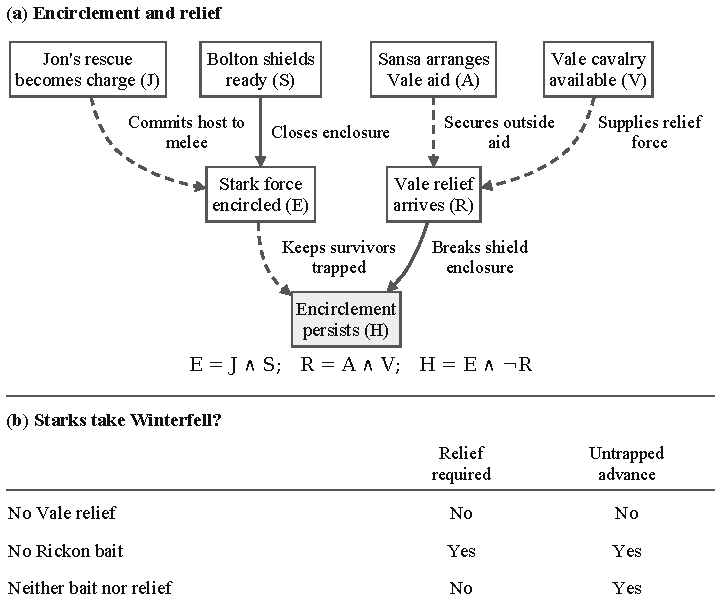
\includegraphics[width=\linewidth]{got/bolton_mechanism_interventions.pdf}
\caption{\BoltonCaption}\label{fig:bolton}
\end{figure}

The scenario comparison concerns what happens next. Let $G$ denote an available Stark field force and $P$ its effective pursuit and advance. The \emph{relief-required} scenario uses $P=G\land R\land\neg H$; the \emph{untrapped-advance} scenario uses $P=G\land\neg H$. In the full model, a gate breach $K$ requires both $P$ and an available Wun Wun $W$, so $K=P\land W$; capture $Y$ follows $Y=K\land P$. All these later mechanisms remain fixed between interventions within each scenario.

\begin{samepage}
Removing timely relief alone leaves the encirclement persistent and prevents capture in both scenarios. Removing Rickon's use as bait alone prevents the modeled exposed advance and still permits capture. The joint intervention removes both bait and relief. Under the bait-to-advance rule, no trap forms, so $H=0$. The relief-required model nevertheless gives $P=0$ and no capture; the untrapped-advance model gives $P=1$ and capture, with other inputs unchanged. This isolates the extra assumption that relief is required even when there is no encirclement to remove.
\par
\end{samepage}

\subsection{Astapor: authority, force and voluntary service}
Obtaining command, breaking armed control and gaining voluntary service are different events in the Astapor map. Figure \ref{fig:astapor} follows the bargain in \ep{S03E03} through the departure in \ep{S03E04}. Its outcome combines the breaking of the masters' immediate armed control with departure of a freed force. Separating these steps explains more than a single claim that Daenerys obtains an army.

Let $O$ be the dragon offer, $B$ the accepted bargain and $C$ command transfer. In panel (a), $B=O$ and $C=B$ retain the counterparties' observed acceptance and implementation as scenario assumptions. In panel (b), $Q$ is the order against the masters and $U$ defeat of their guards, with $U=C\land Q$. Authority provides access to an obedient force, while the order directs that force toward the particular action. Keeping these nodes separate distinguishes having command from exercising it.

\begin{figure}[p]
\centering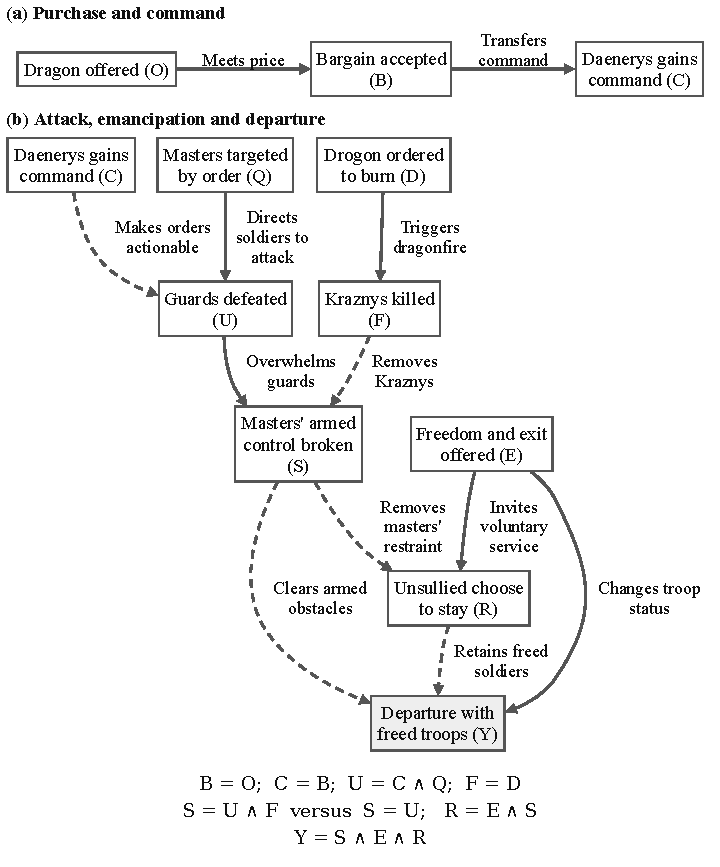
\includegraphics[width=\linewidth]{got/astapor_overview.pdf}
\caption{\AstaporCaption}\label{fig:astapor}
\end{figure}

The parallel dragon route distinguishes the Dracarys order $D$ and the killing of Kraznys by fire $F$, using $F=D$. Let $S$ denote the masters' immediate armed control being broken. The combined-force scenario specifies $S=U\land F$; the alternative specifies $S=U$. Both reproduce the represented events. Preventing the fire strike therefore separates them, whereas withholding the order against the masters prevents the departure outcome in both. The causal question is whether the successful ground action would suffice within this boundary, not whether the depicted dragon attack occurred.

Finally, let $E$ be emancipation with permission to leave, $R$ the troops' decision to remain, and $Y$ departure with a freed army. The scenario uses $R=E\land S$ and $Y=S\land E\land R$. The first rule assumes the observed willingness to stay persists when freedom and immediate security are present; it is not a general law that emancipation produces loyalty. The distinct decision node preserves the meaning of voluntary service even in this simplified deterministic scenario. The outcome ends at departure, excluding subsequent governance of Astapor. The map traces how institutional authority enables military action while keeping freedom and continued service separate.

\subsection{What the portfolio establishes}
Across the six cases, the maps distinguish immediate actions from resources, permissions, beliefs and longer-lived conditions. The northern coalition case, for example, keeps assembling a force separate from securing its crossing and Frey support. The Stark-Lannister case records an allegation about the dagger as information acting on decisions, rather than treating the allegation's content as established fact. These distinctions make different points in an explanation available for inspection.

All 18 selected application questions were executed in both complete scenarios; six, one per case, have different outcomes across those scenarios. The remaining twelve agree within the selected pair. The broader partial families admit both outcome values for every question because many unobserved functional rows were intentionally left unconstrained. These results locate two different tasks: interpreting a mechanism and fully encoding its hypothetical behavior. The complete scenarios expose consequential assumptions; the conservative families show what follows from the weaker encoded constraints alone. Their unresolved answers need not indicate either a misunderstanding of the story or uncertainty inherent in every supporting passage. Agreement within a selected scenario pair is accordingly a sensitivity result, not identification over the broader family.

\clearpage
\section{Discussion and Practical Applications}
The maps connect interpretation to consequences at a level where disagreements can be examined. A reader can trace an arrow to its supporting passage, distinguish a resource from its use, and inspect the joint rule governing an outcome. Alternative rules make differences between explanations concrete, as the Winterfell comparison demonstrates.

This organization supports concrete uses in teaching and narrative analysis. Readers can compare interpretations at a particular mechanism. Editors can inspect whether a claimed consequence has an intervening action or merely follows it in time. A classroom exercise can change a contextual condition and explain why the same action matters differently. These are illustrated capabilities; reader performance has not been measured.

The short-story reassessment separates interpretation from formalization. The controlled Humpty and Wolf outputs expressed all reference joint rules correctly in prose, and Crow expressed three of four. Yet their encodings left behavior unspecified, and Wolf wrongly recorded a timely response. Useful concepts, incomplete equations and genuine factual errors therefore coexist. Direct answers were correct on all twelve questions, while none of the six first-attempt models met executable acceptance. Those generation results remain distinct from the author-reference maps and refined application models.

The application uses one dependent transcription family, with source interpretations assessed by the construction assistant rather than independent adjudicators. Boolean contrasts and fixed backgrounds simplify strategic and institutional processes. The conclusions concern conditional scenarios, not causal probabilities or general narrative understanding. Independent assessment of event, directional and functional support would test the interpretations. Asking readers to locate the assumption behind a changed answer would test explanatory value separately from computational consistency.

\section{Conclusion}
Generative interpretation supplies meaningful events, contextual distinctions and candidate mechanisms; structural modeling makes their joint implications executable. The Crow example shows how an action's importance depends on an alternative route. Six Game of Thrones cases connect interacting decisions, resources and opportunities to particular military and political outcomes. Their maps distinguish mechanisms that a chronological summary can compress, while scenario comparisons expose assumptions responsible for different answers. Connecting passages, readable causal descriptions and fixed structural functions gives readers an account they can trace, question and revise, with a clear relationship between evidence, interpretation and computation.

\section*{Declaration on Generative AI}
Generative AI tools, including OpenAI Codex, assisted manuscript preparation, language editing, coding, figure preparation and consistency checking. Their use in the research method is described in Section \ref{sec:method}. The authors are responsible for the scientific content and final manuscript.
\label{sec:main-end}
\clearpage
\bibliographystyle{plain}
\bibliography{references}
\clearpage
\appendix

\section{Humpty Dumpty: Damage and Repair}\label{app:humpty}
The controlled reference retelling specifies a fall and damage, followed by an unsuccessful attempt by the king's helpers. It does not identify Humpty as an egg. Let $F$ denote falling, $D$ initial damage, $A$ a repair attempt, $E$ availability of an effective method, $R$ successful repair and $Y$ remaining damage. The added rules are
\begin{equation}\label{eq:humpty}
 D=F,\qquad R=D\land A\land E,\qquad Y=D\land\neg R.
\end{equation}
The factual inputs $F=A=1$ and $E=0$ give $D=Y=1$ and $R=0$. Figure \ref{fig:humpty} separates trying to repair from having an effective method and actually succeeding. With the attempt retained, $\doop(E=1)$ gives $R=1$ and $Y=0$. Jointly making a method available and preventing the attempt gives $R=0$ and $Y=1$. Availability and implementation are complementary in this adaptation.

\begin{figure}[htb]
\centering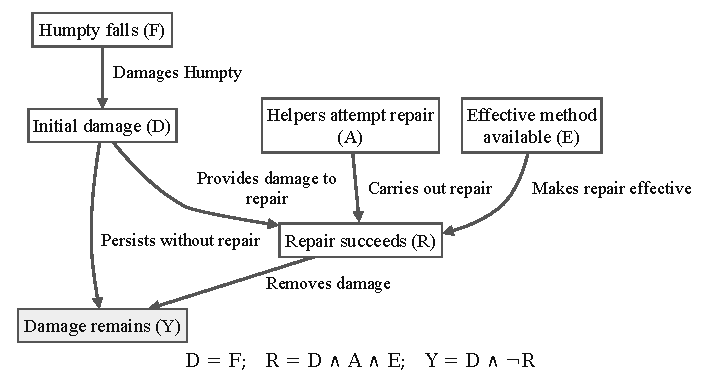
\includegraphics[width=\linewidth]{simple_stories/humpty.pdf}
\caption{\HumptyCaption}\label{fig:humpty}
\end{figure}

Failure by the depicted helpers establishes an unsuccessful repair at the endpoint, not the impossibility of every possible repair. The controlled sentences introduce the explicit success rule; the natural retelling leaves that counterfactual open. Keeping attempted repair, effective repair and remaining damage distinct prevents the observed failure from silently becoming permanent irreparability.

\clearpage
\section{The Boy Who Cried Wolf: Warning and Credibility}\label{app:wolf}
This controlled reference retelling distinguishes earlier false alarms from a new warning about a real wolf. Let $F$ denote the earlier false alarms, $L$ loss of credibility, $W$ a real wolf appearing, $N$ the new warning, $V$ timely village response and $H$ harm to the flock. The adaptation explicitly stipulates
\begin{equation}\label{eq:wolf}
 L=F,\qquad N=W,\qquad V=N\land\neg L,\qquad
 H=W\land\neg V.
\end{equation}
The background fixes the opportunity to warn and the effectiveness of timely help. With $F=W=1$, the boy warns, credibility is absent, villagers do not respond in time, and the flock is harmed. The boy's death is not an event in the specified story.

\begin{figure}[htb]
\centering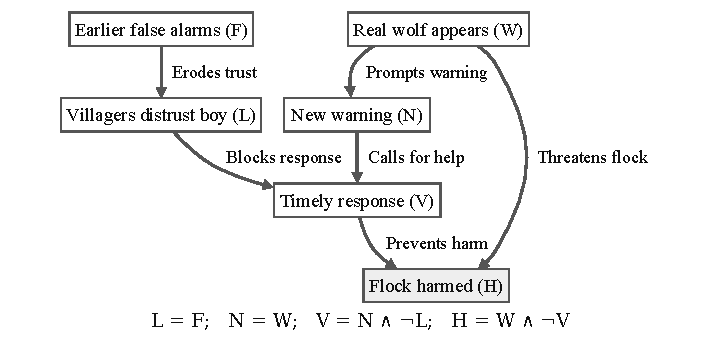
\includegraphics[width=\linewidth]{simple_stories/wolf.pdf}
\caption{\WolfCaption}\label{fig:wolf}
\end{figure}

Preventing the earlier false alarms, $\doop(F=0)$, restores credibility and yields timely help, so $H=0$. The joint intervention $\doop(F=0,N=0)$ also prevents the new warning, giving $V=0$ and $H=1$. Figure \ref{fig:wolf} keeps disbelief distinct from silence: a credible boy who does not warn provides no trigger for the stipulated response. Guaranteed prevention of harm belongs to the adaptation's added rule, rather than being inferred from the natural tale's unhappy outcome.

\clearpage
\section{Assessment of the Short-Story Generations}\label{app:assessment}
None of the six first-attempt models met strict executable acceptance, including after structural normalization. All contained relevant events and relationships. Table \ref{tab:stories} separates supported factual assertions and correctly expressed rules from accepted execution. These assistant reassessment judgments concern semantic correspondence, not literal wording. The three stories, rather than their individual questions or variables, are the descriptive units.

\begin{table}[htbp]
\caption{Semantic content and executable completeness of the unmodified controlled-story generations.}\label{tab:stories}
\centering\small
\setlength{\tabcolsep}{6pt}
\begin{tabular}{@{}lcccc@{}}
\toprule
Story & \shortstack{Supported\\facts} & \shortstack{Correct prose\\rules} & \shortstack{Executable\\acceptance} & \shortstack{Direct\\answers} \\
\midrule
Humpty & 6/6 & 3/3 & No & 4/4 \\
Wolf & 5/6 & 4/4 & No & 4/4 \\
Crow & 8/8 & 3/4 & No & 4/4 \\
\bottomrule
\end{tabular}
\end{table}

The controlled Humpty generation correctly says that repair succeeds exactly when damage, an attempt and an effective method coincide. Its alternative variable names are harmless; an edge making damage a prerequisite for attempting repair needs substantive clarification because the stated prerequisite concerns success. The Wolf generation distinguishes distrust, a new warning, response and harm and correctly describes their joint rules, but records timely response as occurring when the controlled story says it does not. The Crow generation correctly distinguishes initially reachable water from water raised by stones, but adds an intact-pitcher prerequisite to stone addition itself. That changes intermediate behavior when stones are available and the pitcher is not intact, even though the drinking outcome remains zero in that configuration.

Across eleven controlled joint descriptions, nine are compatible with but not entailed by their partial encodings. Two, both in Wolf, conflict with the wrongly recorded response state. Missing encoding in an explicitly specified story is therefore different from uncertainty in its source. A post hoc diagnostic projection retaining supplied rows finds two of Crow's four answers determined and correct, with the other two unresolved. It leaves all four Humpty questions unresolved; Wolf includes one definitely wrong answer. These projections are separate partial-model analyses, not replacements for the original unavailable executed answers. All twelve direct answers and all twelve author-reference executions match the frozen reference answers.

The natural outputs capture useful qualitative content: Humpty's fall and attempted repair, Wolf's loss of credibility and ignored warning, and Crow's rise-to-reach-to-drink sequence. Their supported factual counts are 4/6, 8/8 and 8/8 respectively. Natural Humpty introduces unsupported irreversible damage, whereas the other two preserve gaps about protective help and a leaking pitcher. Equivalent terminology and short causal phrases are assessed in context. Explicit necessity or sufficiency claims still require the quantified behavior they assert. No substantive correction to an archived generation is counted as an initial generation success.

\clearpage
\section{Partial Functions and Coverage}\label{app:uncertainty}
For a fixed graph and finite domains, let $E$ be the evidence and $A$ the additional assumptions. If $C_i(E)$ and $C_i(A)$ are the corresponding local constraints, the admissible functions for event $i$ are
\begin{equation}\label{eq:family}
 \mathcal F_i(E,A)=\{f_i: f_i\text{ satisfies }C_i(E)\text{ and }C_i(A)\}.
\end{equation}
Let $\mathcal M(E,A)$ contain the combinations consistent with all established factual states. For a query $q$ and fixed factual background $u^*$, the outcome set for target $Y$ is
\begin{equation}\label{eq:outcomes}
 \mathcal Y(q)=\{Y_{M,q}(u^*): M\in\mathcal M(E,A)\},
\end{equation}
where $Y_{M,q}(u^*)$ is obtained by replacing only the equations targeted by $q$ in model $M$. A singleton identifies the answer within this family only when exhaustive evaluation or a valid bound establishes that no other outcome is possible. It says nothing about omitted variables or alternative boundaries.

The broad application families fix observed input-output configurations and leave other rows unknown. They may include locally inactive parent links despite qualitative directional support; they are conservative sets of functions, not complete translations of everything the passages imply. Each application mechanism has at most three parents, allowing all local Boolean tables to be considered. Global products range from 65,536 to 8,388,608 functions, so joint search stops at 512 candidates. Every reported broad outcome set is nevertheless certified as $\{0,1\}$: compatible witnesses attain both possible values of the binary target. A complete enumeration is unnecessary to establish that particular set. The two named complete scenarios per case add stronger assumptions and do not exhaust this family.

For formal prose checking, necessity of a positive input requires output zero in every row where that input is zero; sufficiency requires output one in every row where it is one. Exact conjunction and inhibition assertions require their complete stated truth conditions. The retained targeted mutations change a conjunction to disjunction, remove a necessary input or reverse inhibition, and the corresponding quantified checks detect the contradictions. An informal statement that a factor helps does not receive one of these stronger translations without an explicit interpretive justification.
\label{sec:appendices-end}
\end{document}
